\chapter[Metodologia]{Metodologia}
\label{cap-metodologia}

Para cumprir com o objetivo de realizar uma Avaliação do Ecossistema de Startups de Tecnologia do Distrito Federal foi adotada a Metodologia criada por \citeonline{Cukier2015, Kon2014}, uma das primeiras contribuições do Grupo de Pesquisa em Empreendedorismo InovaSampa\footciteref{inovasampa}. 

Este capítulo tem como objetivo descrever a metodologia criada por eles e as adaptações que foram feitas para obter uma visão mais adequada com base nos dados disponíveis no contexto do Distrito Federal. A escolha se deu por recomendação do Orientador deste trabalho, Professor Paulo Meirelles, e por acreditar que ela fornece um bom caminho para obtermos uma visão geral e realista do atual estado do Ecossistema local por ter uma forte integração com empreendedores locais e já ter sido executada em três cidades do mundo: Tel-Aviv \citeonline{Kon2014}, São Paulo \citeonline{MonnaSantos2015} e Nova Iorque \citeonline{Cukier2016}. 

\section{Trabalhos Relacionados}
\label{section:trabalhos_relacionados}

A Endeavor, por meio da Rede Global de Empreendedorismo, elabora o Índice de Cidades Empreendedores\footciteref{indiceglobaldoempreendedorismo} desde 2014 com o objetivo de ajudar ecossistemas locais a crescerem por meio da identificação de fatores que possam ser aprimorados, o Índice pode ser um utilizado como uma espécie de guia para Governantes, Empreendedores engajados com o Ecossistema, Associações, etc. Atualmente ele conta com análise de 32 cidades, em sua maior parte capitais, e a tendência é que por meio da atuação dos Comitês Locais da Rede Global de Empreendedorismo o número de cidades expanda cada vez mais.

\begin{figure}[!htb]
\centering
\includegraphics[width=11cm,angle=0]{figuras/indice_de_cidades_empreendedoras_ranking}
\caption{Ranking do Índice de Cidades Empreendedoras, da Endeavor}
\label{Rotulo}
\end{figure}

A metologia tem como base sete pilares: ambiente regulatório, infraestrutura, mercado, acesso a capital, inovação, capital humano e cultura empreendedora. A maior dificuldade encontrada pelos pesquisadores fora a dificuldade em encontrar dados sistemáticos sobre o Ecossistema brasileiro, por exemplo motivo as principais fontes de dados são bases públicas mas nem sempre estão atualizadas, mas alguns estão sob domínio de terceiros, em sua maior parte entidades privadas, ou precisaram ser criados. 

De acordo com esses índicadores em 2016 Brasília obteve ótimos indicadores de Mercado e Acesso à Capital, mas não se destacou em Ambiente Regulatório, Inovação, Capital Humano e demonstrou resultados muito ruins em Infraestrutura e Cultura Empreendedora. Os resultados e a comparação com Goiânia estão representados na Figura XX.

\begin{figure}[!htb]
\centering
\includegraphics[width=11cm,angle=0]{figuras/indice_de_cidades_empreendedoras_brasilia_e_goiania}
\caption{Análise de Brasília no Índice de Cidades Empreendedoras, da Endeavor}
\label{Rotulo}
\end{figure}

Embora seja a análise mais completa já realizada sobre o Ecossistema Empreendedor de Brasília, o Índice de Cidades Empreendedoras não tem como foco o cenário de Startups e tem como uma forte base análises de dados quantitativos, mas é de altíssima importância para validar alguns dos pontos levantados por este trabalho.

\citeonline{Suresh2012} buscou, por meio de um estudo qualitativo e revisões bibliográficas, mapear quais elementos encorajam as pessoas a seguirem o caminho do Empreendedorismo e encontrou oito fatores essenciais: Suporte Moral, desempenhado pelo seu circulo social, Suporte Financeiro, seja por meio da família, governo, empréstimos ou investimentos, Suporte da Rede, no geral vindo de associações ou redes sociais, Suporte do Governo, Suporte de Tecnologia, desempenhado por centros de pesquisa e encubação, talentos disponíveis no mercado local, etc, Suporte do Mercado, Suporte Social, relacionado principalmente com a aceitação da falha e pelas ações da mídia, e Suporte do Ambiente, relacionado com recursos naturais e condições de clima.

\citeonline{Lemos2011} propôs uma metodologia para avaliação de Ecossistemas de Startups com o viés de apoiar o desenvolvimento de gestão estratética do Empreendedorismo dentro das universidades a partir do modelo de hélice tripla, que defende que para a atração de inovação e o desenvolvimento econômico de uma região cresçam é necessário uma forte integração entre Governo, Universidades e Indústria. Com base em outros autores ele introduz a importância de se adicionar os Empreendedores na equação e trás uma abordagem de análise qualitativa similar a deste trabalho.

\citeonline{Arnaud2009} e \citeonline{Ahmad2007} por meio da OECD definiram três grandes pilares para avaliar o Empreendedorismo em uma região, o primeiro, de Determinantes é composto por indicadores Ambiente Regulatório, Cultura, Pesquisa \& Desenvolvimento e Tecnologia, Acesso à Financiamento, Capacidades Empreendedoras, Condições do Mercado. O segundo pilar, chamado de Performance Empreendedora é composto por indicadores baseados nas empresas e nos empregos da região. O terceiro, de Impacto, estuda dados comos Criação de Empregos, Crescimento Econômico e Redução da Pobreza. No mesmo artigo são indicados diversas fontes e meios para se obter dados sobre esses indicadores.

\citeonline{Arruda2013} realizaram um estudo muito similar à proposta deste trabalhando, analisando o Ecossistema Empreendedor Brasileiro de Startups por meio de uma abordagem mista de estudos Qualitativos, onde foram feitas 30 entrevistas com Empreendedores, Representantes de Instituições de Suporte, Investidores, Pesquisadores e Consultores de 5 estados brasileiros, e Quantitativos, com base nos fatores determinantes definidos por \citeonline{Arnaud2009}. 

Como resultados, obtiveram visões sobre o Modelo Regulatório Brasileiro, as nossas Condições de Mercado, o Acesso a Financiamento, a Criação e Difusão de Conhecimento, a Capacidade e a Cultura Empreendedora e as peculiaridades regionais do Brasil no que tange o Empreendedorismo e o mercado de Startups. O trabalho também lista em anexo todas as variáveis mapeadas para o trabalho e suas fontes, que foram de grande importância para este trabalho. Nas recomendações de trabalho futuro mencionam a dificuldade em conversar sobre experiências de fracasso com os Empreendedores Brasileiros, em especial com aqueles que ainda não alcançaram o sucesso, talvez esse problema se repita no contexto do Distrito Federal.

\citeonline{Sipola2013} mapearam os atores Consumidores, Inovadores, Empreendedores, Capital de Risco, Mercados de Saída(venda) e Indústrias como peças chaves para um Ecossistema de Startups. 

Os Inovadores são importantes por serem os atores responsáveis por mesclar novas e velhas tecnologias com o objetivo de criar algo novo que seja melhor, mais rápido e mais barato. Empreendedores são aqueles que transformam inovações em produtos em financeiramente viáveis e escaláveis. As Indústrias são responsáveis por permitirem que os melhores produtos sejam produzidos e distribuídos em larga escala. Sem os Mecânismos de Saída não seria possível atrair Capital de Risco e manter o ciclo de expansão e crescimento de negócios existentes e maduros e investimentos em novos negócios funcionando. E, por fim, todo esse ciclo tem como seu ponto central o Consumidor, sem ele, ou ela, o Empreendedorismo e as Inovações perderiam seus propósitos.

\citeonline{Kutt2013}, por meio de uma análise quantitativa de diversas bases de dados locais e globais fez uma comparação do Ecossistema de Startups da Estônia em um contexto internacional, comparando-o como Finlândia, Taiwan, Israel, Coreia e Singapura. O autor também fez um estudo por meio da análise de dados de redes sociais para obter uma visualização das estruturas sociais do Ecossistema da Estônia e identificar como os atores se conectam entre si.

\citeonline{Hermann2015} por meio do ``The Global Startup Ecosystem Ranking'' e da Compass realizaram um estudo dos principais Ecossistemas de Startups do mundo com base em seis pilares principais: Performance, Financiamento, Alcance de Mercado, Talento, Experiência em Startups e Índice de Crescimento. O ranking de 2015 está representado na Figura XX, cada coluna representa um pilar e os valores numéricos em cada uma delas representam a posição de cada Ecossistema no pilar correspondente. 

\begin{figure}[!htb]
\centering
\includegraphics[width=11cm,angle=0]{figuras/global_startup_ecosystem_ranking}
\caption{Ranking do Global Startup Ecosystem Ranking criado pela Compass}
\label{figure:global_startup_ecosystem_ranking}
\end{figure}

Esse é um dos trabalhos disponíveis mais extensos que já foram realizados no contexto de Ecossistemas de Startups, cerca de 11 mil participantes de 40 Ecossitemas participaram da pesquisa por meio de questionários, mais de 200 especialistas de 25 países foram entrevistados e aproximadamente 35 mil empresas de tecnologia tiveram seus dados estudados pela Compass. Também foram avaliadas diversas bases de dados públicas. Ele também teve uma grande contribuição na metodologia utilizada como base para este trabalho, criada por \citeonline{Cukier2015, Kon2014}, mas, como explorado em \ref{subsection:vantagens_e_desvantagens} não será de muita utilidade no contexto do Distrito Federal por ter como referência a cidade de São Paulo.

\citeonline{Kon2014}, em um dos primeiros artigos do grupo InovaSampa, relatam que foram encontrados poucos trabalhos que criam um arcabouço conceitual ou visões de Ecossistemas de Startups, mas mencionam \citeonline{Chorev2006} por terem mapeado alguns fatores críticos para o sucesso de uma Startup com base nas visões de 9 Empreendedores, divididos em grupos de acordo com a maturidade de suas Startups, e 3 Investidores. Os fatores de sucesso estão representados na Figura XX.

\begin{figure}[!htb]
\centering
\includegraphics[width=11cm,angle=0]{figuras/success_or_failure_factors_model}
\caption{Fatores que influenciam o sucesso de uma Startup criado por \citeonline{Chorev2006}}
\label{figure:success_or_failure_factors_model}
\end{figure}

Kon também menciona o trabalho de \citeonline{Frenkel2014}, por criar um mapa visual de um Ecossistema de Inovação muito similar ao do trabalho realizado pelo InovaSampa porém obtendo os dados com a realização de um workshop e não diversas entrevistas individuais, e o modelo para avaliação de Inovação criado por \citeonline{Belitz2011} representado pela Figura XX. 

\begin{figure}[!htb]
\centering
\includegraphics[width=11cm,angle=0]{figuras/innovation_model}
\caption{Modelo de Avaliação de Inovação por \citeonline{Belitz2011}}
\label{figure:innovation_model}
\end{figure}

Por ter sido uma imagem extraída do artigo citado e criada pelos autores mencionados, é importante ressaltar que a letra ``D'' representa Demanda, a letra ``E'' representa Educação, as letras ``R\&D'' representam Pesquisa e Desenvolvimento, a letra ``N'' representa ``Networking'', a letra ``I'' representa Implementação, as letras ``S\&T'' representam Ciência e Tecnologia e as letras ``SC'' representam Capital Social. \citeonline{Kon2014} enfatiza que muitos desses fatores estão presentes em seu arcabouço conceitual de um Ecossistema de Startups, com a diferença em que seu estudo foram explorados o relacionamento entre esses fatores ao invés de trata-los de forma isolada.

\section{A Metodologia do InovaSampa}
\label{section:metodologia_do_inovasampa}

\subsection{Desvantagens e Vantagens}
\label{subsection:vantagens_e_desvantagens}

Até a publicação deste trabalho as três cidades que foram objetos de estudo do InovaSampa, e que contribuiram para a construção dessa Metodologia, são conhecidas globalmente como grandes centros empreendedores e dispõem de uma vasta quantidade de dados nacionais e globais disponíveis, o que não condiz com a realidade de Ecossistemas menores, como o do Distrito Federal, e torna alguns dos fatores ou medidas sugeridos fora de contexto com o que temos disponível. Infelizmente não existe produção de dados sistemáticos sobre os diversos ambientes empreendedores no Brasil e o acesso à informações confiáveis e atualizados é um desafio.

Para contornar esse problema, e trazer melhorias à Metodologia para que ela possa ser melhor utilizada no contexto de outras cidades brasileiras que também carecem de dados e querem conhecer e desenvolver seus Ecossistemas, alguns fatores foram excluídos ou adaptados para se adaptarem às informações disponíveis. Tudo está descrito na sessão \ref{subsection:fatores_que_formam_um_ecossistema}.

A maior vantagem da Metodologia proposta se dá por ter, como sua maior base, dados obtidos a partir das visões daqueles que melhor o entendem e lidam com o Ecossistema de Startups local - os próprios empreendedores. Ao permitir que os fatores sejam mensurados de acordo com esses dados torna-se possível visualizar quais são as características mais fortes e fracas do Ecossistema em estudo como um todo e compara-los direta ou indiretamente com outros Ecossistemas.

\subsection{Técnicas Utilizadas}
\label{subsection:tecnicas_utilizadas}

Toda a metodologia foi construida com base nas técnicas de Pesquisa Qualitativa e na Teoria Fundamentada em Dados por oferecerem a possibilidade de obter dados a partir das visões daqueles que melhor o entendem e lidam com o Ecossistema de Startups local e seus pontos fortes e fracos todos os dias - os próprios empreendedores - por meio de entrevistas, dessa forma é possível valorizar e obter respostas a partir de suas experiências individuais.

! TO-DO: estudar sobre pesquisa qualitativa e teoria fundamentada em dados para embasar melhor essa subseção !

\subsection{Fatores que formam um Ecossistema}
\label{subsection:fatores_que_formam_um_ecossistema}

Após vasta pesquisa bibliográfica e entrevistas com mais de 50 pessoas chaves para os Ecossistemas de Tel-Aviv e São Paulo foram definidos cerca de 21 fatores que os compõem e fazem parte do Arcabouço Teórico de um Ecossistema, descrito na subseção \ref{subsection:arcabouco_conceitual_e_modelo}. 

\begin{description}

  \item [Estratégias de Saída:] Quando falamos de Estratégias de Saída falamos de formas de transformar uma empresa em capital, em converter ações em dinheiro real. Investidores não estão em busca de empresas com modelos de negócios conservadores e com taxas de crescimento controladas e tímidas, eles estão em busca de empresas que vão obter uma taxa de crescimento muito alta e proporcionar possibilidades de saída rápido, geralmente com a venda da empresa ou por meio da abertura de capital na bolsa de valores, para que eles possam concretizar o investimento e lucrar. Para um investidor nada é pior do que ter o seu dinheiro investido em uma empresa sem prospecções de saída, mesmo que a empresa demonstre crescimento constante. Se não há como converter o investimento em dinheiro no bolso ele terá sido em vão. Um Ecossistema com diversas opções e uma quantidade alta de saídas bem sucedidas certamente atrairá muitos investidores e contribuirá para o seu crescimento. Elemento(s) relacionado(s) no arcabouço: Startup, Investimentos, Empresas Estabelecidas.

  \item [Mercado Global:] Porcentagem de Startups no Ecossistema com abrangência de mercado global. Elemento(s) relacionado(s) no arcabouço: Mercado.

  \item [Empreendedorismo nas Universidades:] Porcentagem de ex-alunos que fundaram uma empresa em até 5 anos após a graduação. Elemento(s) relacionado(s) no arcabouço: Universidades, Centros de Pesquisa e Educação.

  \item [Número de Startups:] Número de Startups em atividade por ano de acordo com fontes de dados confiáveis em um dado ano. Elemento(s) relacionado(s) no arcabouço: Mercado.

  \item [Acesso ao investimento em US\$ por ano:] Quantidade de dinheiro investido em Startups locais, em dólares americanos, de acordo com fontes confiáveis em um dado ano. Elemento(s) relacionado(s) no arcabouço: Opções de Investimento. 

  \item [Investidores Anjo: ]

  \item [Acesso ao investimento em quantidade de negócios realizados:] Contagem simples de quantos investimentos foram realizados em Startups locais, independente do valor, de acordo com fontes confiáveis em um dado ano. Elemento(s) relacionado(s) no arcabouço: Opções de Investimento.

  \item [Qualidade dos Mentores:] Um mentor de qualidade é um empreendedor experiente, alguém que já viveu os problemas que o novo empreendedor está passando e entende perfeitamente a sua situação, ninguém melhor para orienta-lo do que alguém que já passou por problemas similares ou iguais. Elemento(s) relacionado(s) no arcabouço: Empreendedor.

  \item [Burocracia:] Em sua maioria envolve o ambiente regulatório do Ecossistema Local e representa o quanto a burocrácia impacta as Startups como, por exemplo, envolvendo o tempo, custo médio e a complexidade tributária para se abrir e manter uma empresa. Elemento(s) relacionado(s) no arcabouço: Ambiente Regulatório.

  \item [Gastos com Impostos:] Baseado no ranking de impostos entre países criado por \citeonline{schwab2015}. Elemento(s) relacionado(s) no arcabouço: Ambiente Regulatório, Mercado. 

  \item [Incubadoras e Parques Tecnológicos:] Representação da quantidade de incubadoras e parques tecnológicos presentes no Ecossistema. Elemento(s) relacionado(s) no arcabouço: Incubadoras.

  \item [Qualidade das Aceleradoras:] Porcentagem das Startups que passaram por algum programa de Aceleração ou Incubação e se estabeleceram bem no mercado ou avançaram com sucesso para a fase de captação de investimento de terceiros. Elemento(s) relacionado(s) no arcabouço: Aceleradoras, Incubadoras e Parques Tecnológicos.

  \item [Presença de Empresas de Alta Tecnologia:] Quantidade de empresas de alta tecnologia presentes no Ecossistema. Elemento(s) relacionado(s) no arcabouço: Empresas Estabelecidas. (mas qual o parâmetro para considerar uma empresa de alta tecnologia? talvez uma multinacional ou empresa com valor acima de X milhões)

  \item [Influência de Empresas já estabelecidas:] A quantidade de empresas estabelecidas e engajadas em movimentar o Ecossistema por meio de eventos, líderança, mentoria e apoio, investimentos ou programas de aceleração para Startups locais. Elemento(s) relacionado(s) no arcabouço: Eventos, Empresas Estabelecidas, Aceleradoras, Empreendedores.

  \item [Qualidade do Capital Humano:] Fator baseado no índice de talentos definido por \citeonline{Hermann2015}. Elemento(s) relacionado(s) no arcabouço: Empreendedor, Educação.

  \item [Valores Culturais para o Empreendedorismo:] Fator baseado no índice de suporte cultural definido por \citeonline{Acs2016}. Elemento(s) relacionado(s) no arcabouço: Cultura, Sociedade e Família.

  \item [Processos de Transferência de Tecnologia:] Índice baseado nos fatores de Inovação e Sofisticação definidos por \citeonline{schwab2015}. Elemento(s) relacionado(s) no arcabouço: Universidades, Centros de Pesquisa e Ambiente Regulatório.

  \item [Conhecimento das Metodologias:] Porcentagem de Empreendedores que possuem conhecimento de diversas metodologias comumente utilizadas pelo mercado como Métodos Ágeis, Lean Startup, Canvas, Design Thinking, etc. Por ser um fator difícil de ser mensurado, os autores da Metodologia sugerem utilizar a quantidade de eventos relacionados no Ecossistema. Elemento(s) relacionado(s) no arcabouço: Metodologias.

  \item [Atores da Mídia com foco no Empreendedorismo:] A participação da mídia é muito importante para a promoção do Ecossistema como um todo e de seus Empreendedores, portanto a presença de profissionais engajados e que entendam o contexto do mercado local é de extrema importância. Elemento(s) relacionado(s) no arcabouço: Mídia.

  \item [Dados do Ecossistema e Pesquisas:] As universidades e os institutos de pesquisas são peças triviais em um Ecossistema de Startups, em especial por constantemente levantarem questões, respostas, informações e pontos que devem ser aprimorados em prol de um ambiente mais maduro e preparado. Também é importante que os dados sejam amplamente acessíveis, de forma que diversas peças interessadas possam ter acesso para embasarem suas ações, identificarem pontos em que podem contribuir ou atraírem mais pessoas para o Ecossistema. Elemento(s) relacionado(s) no arcabouço: Centros de Pesquisa, Governo.
  
  \item [Gerações do Ecossistema:] De tempos em tempos o Ecossistema possui uma nova leva de Empreendedores se destacando no mercado e, conforme sua maturidade aumenta, novas gerações são inspiradas, influenciadas e apoiadas pelas anteriores. Elemento(s) relacionado(s) no arcabouço: Empreendedor, Sociedade.  

  \item [Eventos relacionados à Startups:]     
\end{description}

Com o objetivo de classifica-los entre níveis para facilitar as comparações e o cálculo final da maturidade do Ecossistema foram definidas as seguintes métricas para cada um dos fatores representados na Tabela \ref{tabela:metricas_de_classificacao_dos_fatores}, vale ressaltar que os fatores que contém o símbolo \"*\" antes de seu nome são os fatores essenciais, os restantes são os fatores derivados.

\begin{table}[!htb]
\centering
\caption{Métricas de classificação dos Fatores que compõem um Ecossistema}
\label{tabela:metricas_de_classificacao_dos_fatores}
\begin{tabular}{llll}
Fator                                                      &     L1     &     L2     &     L3      \\
Estratégias de Saída*                                      &     00     &     01     &    >=2      \\
Mercado Global*                                            &    <10\%   &   10-40\%  &    >40\%    \\
Empreendedorismo nas Universidades*                        &    <02\%   &   02-10\%  &    >10\%    \\
Qualidade de Mentores                                      &    <10\%   &   10-50\%  &    >50\%    \\
Burocracia                                                 &    >40\%   &   10-40\%  &    <10\%    \\
Gastos com impostos                                        &    >50\%   &   30-50\%  &    <30\%    \\
Qualidade das Aceleradoras                                 &    <10\%   &   10-50\%  &    >50\%    \\
Acesso à investimento em US\$ por ano                      &    <200M   &   200M-1B  &    >1B      \\
Qualidade do Capital Humano                                &    >20th   &   15-20th  &    <15th    \\
Valores Culturais para o Empreendedorismo*                 &    <0.5    &   0.5-0.75 &    >0.75    \\
Processos de Transferência de Tecnologia                   &    <4.0    &   4.0-5.0  &    >5.0     \\
Conhecimento das Metodologias                              &    20\%    &   20-60\%  &    >60\%    \\
Atores da Mídia com foco no Empreendedorismo               &    <03     &   03-05    &    > 05     \\
Eventos relacionados à Startups*                           &   monthly  &   weekly   &    daily    \\
Dados do Ecossistema e Pesquisas*                          &    nada    & parcial    & disponíveis \\
Gerações do Ecossistema*                                   &     00     &    0.1     &    02       \\
Número de Startups*                                        &    <200    &   200-1k   &    >1k      \\
Acesso à investimento em quantidade de negócios/ano        &    <50     &   50-300   &    >300     \\
Acesso à investimento anjo em quantidade/ano*              &    <05     &   05-50    &    >50      \\
Incubadoras e Parques Tecnológicos                         &     01     &    02-05   &    >5       \\
Presença de Empresas de Alta Tecnologia*                   &    <02     &   02-10    &    >10      \\
Influência de Empresas já estabelecidas                    &    <02     &   02-10    &    >10      \\
\end{tabular}
\end{table}

\subsection{Versão Enxuta do Modelo de Avaliação}
\label{subsection:versao_enxuta_do_modelo_de_avaliacao}

Também foi desenvolvido uma versão mais enxuta do Modelo, com foco em apenas oito fatores ao invés de 21. Os parâmetros utilizados estão representados na Figura XX e a importância de cada um dos fatores na Figura XX.

\begin{figure}[!htb]
\centering
\includegraphics[width=11cm,angle=0]{figuras/short_version_maturity_model}
\caption{Parâmetros utilizados pela versão enxuta do Modelo de Maturidade por \citeonline{Cukier2016}}
\label{figure:short_version_maturity_model}
\end{figure}

\begin{figure}[!htb]
\centering
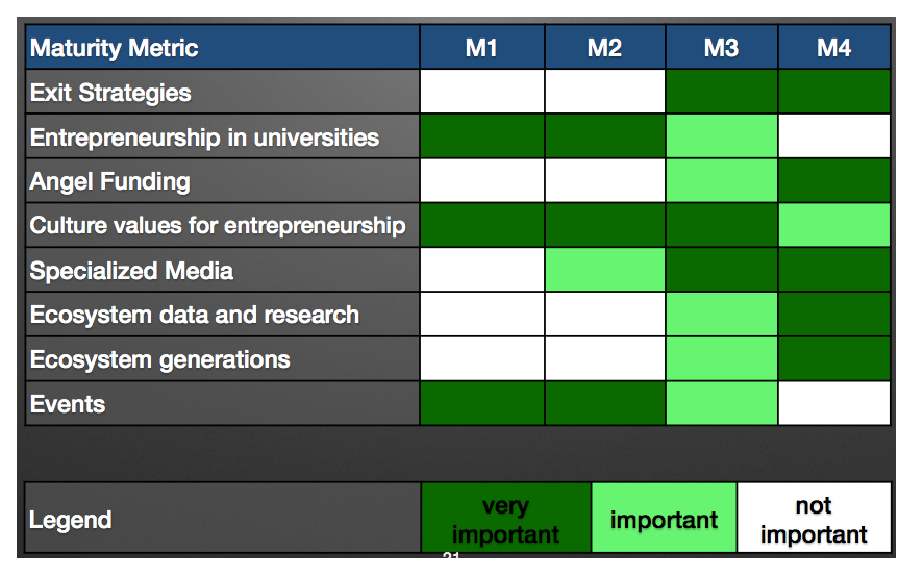
\includegraphics[width=11cm,angle=0]{figuras/metrics_importance}
\caption{Importância das Métricas citadas para cada um dos níveis de maturidade por \citeonline{Cukier2016}}
\label{figure:metrics_importance}
\end{figure}

\subsection{O arcabouço conceitual e o Mapa de um Ecossistema}
\label{subsection:arcabouco_conceitual_e_modelo}

Com base nesses mesmos fatores descritos na subseção \ref{subsection:fatores_que_formam_um_ecossistema} e na relevância de cada um deles de acordo com a visão das pessoas que compõem o próprio Ecossistema e nas informações disponibilizadas por outras pesquisadores ou bases de dados foi elaborado um arcabouço conceitual de um Ecossistema, representado pela Figura 01. Na Figura 02 está representado o Mapa do Ecossistema de Tel-Aviv, Israel, e na Figura 03 o Mapa do Ecossistema de São Paulo, ambos tendo como base o mesmo arcabouço conceitual.

\begin{figure}[!htb]
\centering
\includegraphics[width=11cm,angle=0]{figuras/arcabouco_teorico_de_um_ecossistema}
\caption{Arcabouço Conceitual de um Ecossistema de Startups}
\label{figure:arcabouco_teorico_de_um_ecossistema}
\end{figure}

\begin{figure}[!htbp]
\centering
\includegraphics[width=13cm,angle=0]{figuras/mapa_conceitual_tel_aviv}
\caption{Mapa do Ecossistema de Tel-Aviv, Israel}
\label{figure:mapa_conceitual_tel_aviv}
\end{figure}

\begin{figure}[!htbp]
\centering
\includegraphics[width=13cm,angle=0]{figuras/mapa_conceitual_sao_paulo}
\caption{Mapa do Ecossistema de São Paulo, Brasil}
\label{figure:mapa_conceitual_sao_paulo}
\end{figure}

\subsection{Os níveis de maturidade de um Ecossistema}
\label{subsection:niveis_de_maturidade_de_um_ecossistema}

Além de elaborar o mapa do ecossistema a Metodologia tem como um dos seus objetivos classificar Ecossistemas entre quatro diferentes níveis de maturidade. Os níveis são os seguintes:

\begin{description}
  \item [Nascente (M1):] quando há um Ecossistema com algumas Startups presentes no mercado, alguns investimentos concretizados e algumas iniciativas com o objetivo de estimular ou fomentar o Ecossistema sendo realizadas mas não há reconhecimento ou as Startups não possuem representatividade nos índices de geração de emprego e renda da região.

  \item [Crescente (M2):] quando há algumas Startups estabelecidas como empresas sólidas e o Ecossistema como um todo possui representatividade notável na economia regional e nos índices de empregos. Para se enquadrar como Crescente todos fatores essenciais e cerca de 30\% dos fatores derivados deverão ser classificadas como nível L2.

  \item [Maduro (M3):] quando existem algumas centenas de Startups em atividade, sendo algumas reconhecidas internacionalmente e com negócios realizados globalmente, um histórico relevante de investimentos concretizados dentro do Ecossistema e pelo menos uma geração de empreendedores bem sucedidos que se tornaram líderes, mentores, referências e investidores-anjo para os novos empreendedores, ajudando-os a crescer. Além dessas características, para ser considerado como um Ecossistema Maduro, todos os fatores essenciais e pelo menos 50\% dos fatores derivados devem ser classificadas como nível L2 e, no mínimo, 30\% de todos os fatores devem estar enquadrados no nível L3.

  \item [Sustentável (M4):] quando o número de Startups em atividade e de aquisições e/ou investimentos dentro do Ecossistema ultrapassam a casa dos milhares, há no mínimo duas gerações de empreendedores bem sucedidos que iniciaram suas carreiras com Startups de tecnologia presentes, uma rede de empreendedores comprometidos com o desenvolvimento do Ecossistema à longo prazo, um ambiente inclusivo com muitos eventos envolvendo temáticas que fomentem a cultura empreendedora e o mercado local e a presença de uma alta quantidade de profissionais de alta qualidade técnica. Para possuir esse estágio de maturidade, todos os fatores essenciais devem ser classificados como nível L3 e pelos menos 80\% dos fatores derivados também como nível L3.
\end{description}

\section{Aplicação da Metodologia e Protocolo}
\label{section:aplicacao_da_metodologia}

A aplicação da Metodologia foi dividida em três etapas:

\begin{enumerate}
  \item Entrevistas e Observações
  \item Codificação dos Dados
  \item Análises e Conclusões
\end{enumerate}

A primeira, de Entrevistas e Observações, se deu por meio da observação de diversos eventos que movimentam o Ecossistema de Startups do Distrito Federal e das pessoas que o compõem e por meio de entrevistas individuais com pessoas atuantes no Ecossistema com objetivo de entender seu contexto pessoal e profissional, bem como suas visões sobre a realidade e as dinâmicas do Ecossistema como um todo, quais os seus pontos fortes e fracos, seus maiores problemas, como diversas instituições e pessoas interagem entre si afim de fomenta-lo e quais ações poderiam ser tomadas afim de melhora-lo.

Com a Codificação dos Dados todas as informações levantadas pela primeira etapa foram catalogadas em tabelas com o objetivo de se tornarem referências para as etapas de Análises e Conclusões e futuras pesquisas bem como documentar todo o processo que foi realizado. 

Com as Análises dos dados e sua adequação nos fatores pré-definidos será possível mensurar a maturidade do Ecossistema com o objetivo de gerar as Conclusões da pesquisa, que se concentrarão em explicitar o atual estágio do Ecossistema de acordo com a Metodologia utilizada, em realizar comparações com outros Ecossistemas e identificar uma série de ações que podem ser tomadas para aprimorar determinados pontos.

\subsection{Perguntas de Pesquisa}
\label{subsection:questoes_de_pesquisa}

As perguntas da subseção anterior visam responder as seguintes Questões que representam o objetivo final deste trabalho como um primeiro passo para conhecer, mapear e mensurar o Ecossistema de Startups do Distrito Federal.

\begin{itemize}
  \item Pergunta de Pesquisa 1: Quais são as características socioculturais de Brasília que promovem ou inibem o espirito empreendedor?
  \item Pergunta de Pesquisa 2: Quais são os mecânismos institucionais de Brasília que promovem ou dificultam o Empreendedorismo?
  \item Pergunta de Pesquisa 3: Quais são os mecânismos educacionais de Brasília que promovem o Empreendedorismo?
  \item Pergunta de Pesquisa 4: Como os fatores tecnológicos influenciam o sucesso ou fracasso das Startups de Brasília? Qual o papel executado pela comunidade e pelo Software Livre?
  \item Pergunta de Pesquisa 5: Qual a relação do empreendedor de Brasília com as opções de investimento disponíveis e como elas influenciam o Ecossistema?
  \item Pergunta de Pesquisa 6: Quais ações devem ser tomadas no Ecossistema de Brasília para que ele cresça?
\end{itemize}

\subsection{Escolha dos Entrevistados}
\label{subsection:escolha_dos_entrevistados}

É de extrema importância que os entrevistados sejam pessoas atuantes e bem conectados com o Ecossistema de Startups do Distrito Federal como um todo e, em sua maior parte, Empreendedores mas também Professores, Servidores Públicos, Investidores, Representantes de Incubadoras e Aceleradoras e Estudantes. 

Para a escolha dos Entrevistados fora aplicada a metodologia bola de neve. Primeiramente foram definidos algumas pessoas com alto histórico de contribuição ao Ecossistema e que faziam parte da rede de contatos das pessoas envolvidas com a Pesquisa e ao fim de cada entrevista ou conversa informal foram pedidas recomendações de quais pessoas deveriam fazer parte deste pesquisa por serem referências para o Ecossistema, bem como, se possível, solicitado uma introdução entre essas pessoas. 

A meta é que sejam entrevistados cerca de 30 pessoas divididos entre líderes e fomentadores do Ecossistema, empreendedores, membros da comunidade acadêmica, representantes de incubadoras e aceleradoras, investidores e agentes públicos envolvidos com políticas públicas de fomento ao empreendedorismo. 

Até o momento a listagens de pessoas a serem convidadas para a entrevista e justificativa pode ser encontrada em: http://bit.ly/1X9Y33K

\subsection{Condução das Entrevistas}
\label{subsection:conducao_das_entrevistas}

Todas as entrevistas devem ser realizadas, preferencialmente, no ambiente profissional dos Empreendedores de forma a mantê-los à vontade. Caso não seja possível, ela poderá ser conduzida em ambiente escolhido pelo empreendedor, como bibliotecas, cafeterias ou eventos e apenas em último caso de forma remota. Elas também serão gravadas em aúdio caso haja consentimento do empreendedor afim de facilitar a fase de Codificação dos Dados.

As entrevistas não devem ser muito longas, preferencialmente não sendo extendidas por mais de uma hora e meia. Para guiar o Entrevistador foram estabelecidas uma série de Perguntas que devem ser realizadas aos Entrevistados com o objetivo de obter respostas que respondam às Questões de Pesquisa estabelecidas e nos forneçam uma visão geral do Ecossistema. As Questões de Pesquisa foram as mesmas definidas pelo Professor Fabio Kon mas as Perguntas foram adaptadas à realidade do Distrito Federal.

Não necessariamenteas entrevistas devem seguir de forma rígida todas as perguntas definidas no roteiro, o entrevistador poderá ter liberdade de conduzi-la como bem entender. Como a entrevista será conduzida ou a linguagem utilizada não é de grande importância, desde que a maior parte das questões sejam respondidas, mesmo que de forma indireta. Há a possibilidade de que o próprio entrevistado responda algumas delas durante outras perguntas. 

\subsection{Roteiro de Entrevista e Perguntas}
\label{subsection:roteiro_de_entrevista_e_perguntas}

\begin{description}

  % Perguntas com o objetivo de quebrar o gelo e deixar tanto entrevistado quanto entrevistador mais confortáveis ! 

  \item [Pergunta 01:] Você poderia me contar um pouco da sua trajetória? Como se tornou um empreendedor? Já se envolveu com outras Startups/Empresas antes? Quais as suas motivações? 

  \item [Pergunta 02:] Falando sobre a sua Startup, o que ela faz? O que te motivou a cria-la? Em que fase está, hoje? Como foi o começo? O que mais te ajudou? O que foi mais difícil? Já tem clientes? Como foi o processo para capta-los?

  %! A partir dessa pergunta tento obter algumas informações sobre os fatores socioculturais do Ecossistema!

  \item [Pergunta 03:] Quais erros você já cometeu na sua vida empreendedora? Se pudesse voltar no tempo, o que faria de diferente? Acredita que os erros foram importantes na sua trajetória? Como as pessoas ao seu redor enxergam os erros? 

  \item [Pergunta 04:] Na sua visão, quais são as características essenciais para um Empreendedor na área de tecnologia? Você enxerga essas características nas pessoas da área de tecnologia(empreendedores, profissionais, estudantes, etc) do Distrito Federal? Quais são as principais motivações daqueles que já empreendem com Startups no DF? Dinheiro? Fama? Autoestima? Necessidade?
  
  \item [Pergunta 05:] Quais são as características de times de sucesso? Diversidade é importante? Como? Qual seria a combinação ideal (backgrounds) de um time de fundadores? Qual a sua visão sobre os times das Startups que são formadas no Distrito Federal?

  %! A partir dessa pergunta tento entender como e se o Ecossistema se conecta !

  \item [Pergunta 06:] Qual é a relação da sua Startup e a sua relação, como um Empreendedor, com o Ecossistema do Distrito Federal? Acredita que de alguma forma o Ecossistema poderia te dar suporte para os desafios que vem enfrentando no momento ou já enfrentou?

  \item [Pergunta 07:] Como os membros do Ecossistema de Startups do Distrito Federal interagem e colaboram entre si?

  \item [Pergunta 09:] Como você lida com as dificuldades técnicas e pessoais do seu time? Alguma vez o Ecossistema contribuiu com a formação e o crescimento da sua Startup ou com a resolução de problemas/desafios técnicos? Você já contribuiu ou ajudou alguma outra Startup ou Empreendedor? De forma geral, há troca de experiência entre empreendedores e empresas no Distrito Federal? 

  \item [Pergunta 08:] Como você classificaria a presença de empresas de tecnologia já consolidadas no Ecossistema? Elas de alguma forma apoiam, investem ou influenciam os que estão começando?  

  \item [Pergunta 10:] Quais são os fatores que desencorajam ou criam barreiras para o empreendedor iniciar ou chegar ao sucesso no Distrito Federal? E os que encorajam?

  %! Tentando identificar fatores educacionais que fomentam o Ecossistema !

  \item [Pergunta 11:] Qual o papel da Educação na formação do Empreendedor e no Ecossistema do Distrito Federal? Você pode indicar iniciativas educacionais que alimentam ou nutrem o espírito empreendedor nos brasilienses? Quais elementos poderiam ser melhorados na formação educacional dos jovens com objetivo de fomentar o empreendedorismo no Distrito Federal? Para você, houve algum momento específico na sua formação que foi essencial para a sua formação como Empreendedor?

  %! O Fernando Nandico, um dos empreendedores mais experientes do Distrito Federal, relatou de que não considera saudável criar Startups utilizando linguagens modernas em Brasília, como Rails, pela falta de profissionais capacitados. Aqui, segundo ele, é mais interessante trabalhar com Java, PHP, etc. Quero captar a visão de outros players com essas duas perguntas!

  \item [Pergunta 12:] Como aspectos tecnológicos como linguagens de programação, frameworks, software livre, etc influenciam no sucesso ou fracasso das Startups no Distrito Federal? Como esses fatores no contexto do Distrito Federal se comparam com a realidade de outros Ecossistemas? 

  \item [Pergunta 13:] Qual o nível de qualidade dos profissionais da área de Tecnologia do Distrito Federal? Você possui dificuldade para atrai-los? Acredita que algo poderia poderia ser feito para melhorar a oferta e a qualidade de profissionais?
  
  \item [Pergunta 14:] Como aspectos metodológicos(ágeis, lean startup, customer development, canvas, etc) influenciam no sucesso ou fracasso das Startups do Distrito Federal? Quais práticas vocês utilizam? Como elas impactaram seus negócios? Há algo que não funcionou bem? Como esses fatores no contexto do Distrito Federal se comparam com a realidade de outros Ecossistemas?

  %! Tentando entender os mecânismos institucionais do Distrito Federal !

  \item [Pergunta 16:] Que ações em relação ao Ambiente Regulatório você acredita que deveriam ser tomadas para apoiar o empreendedor do Distrito Federal?

  \item [Pergunta 17:] Há algum mecânismo institucional no Distrito Federal que promove o empreendedorismo? Legislações, ações de universidades, agências e programas do governo, fundos de investimento, ONGs, etc. Você se beneficiou por algum deles? Como os classifica? Algo que poderia ser aprimorado? Considera o governo local como um apoiador do Empreendedorismo?

  \item [Pergunta 15:] Quais fontes de capital estão disponíveis no Distrito Federal? Como você classifica a presença e as ações de investidores, aceleradoras e incubadoras no Distrito Federal? Já se relacionou com algum? Como foi a experiência?

  %! Fechamento da entrevista !
  
  \item [Pergunta 20:] Quais são os elementos chave para um ecossistema de Startups vibrante e saudável? Como você descreveria e classificaria o nosso Ecossistema? Quais os nossos pontos fortes e fracos? Algum Ecossistema ao redor do mundo que seja similar ao nosso?

  \item [pergunta 19:] E o que tem sido feito no Distrito Federal para estimular o Ecossistema de Startups? O que mais precisa ser feito?
\end{description}

\subsection{Codificação e Interpretação dos Dados}
\label{subsection:codificacao_e_interpretacao_dos_dados}

Após a realização de cada Entrevista a codificação dos dados será feita utilizando um software CAQDAS(Computer-Assisted/Aided Qualitative Data Analysis Software), preferencialmente de Código Aberto e Gratuito, com o objetivo de facilitarem o trabalho de transcrição e análise de conteúdo. 

%! RQDA e MaxQDA parecem ser os mais adequados, porém o segundo é pago ! 
%! TO-DO: Estudar Miles Huberman sobre fases de análises qualitativas de dados !